\subsection{Stromquellen, elektromotorische Kraft, Urspannung, Klemmspannung}

\begin{center}
	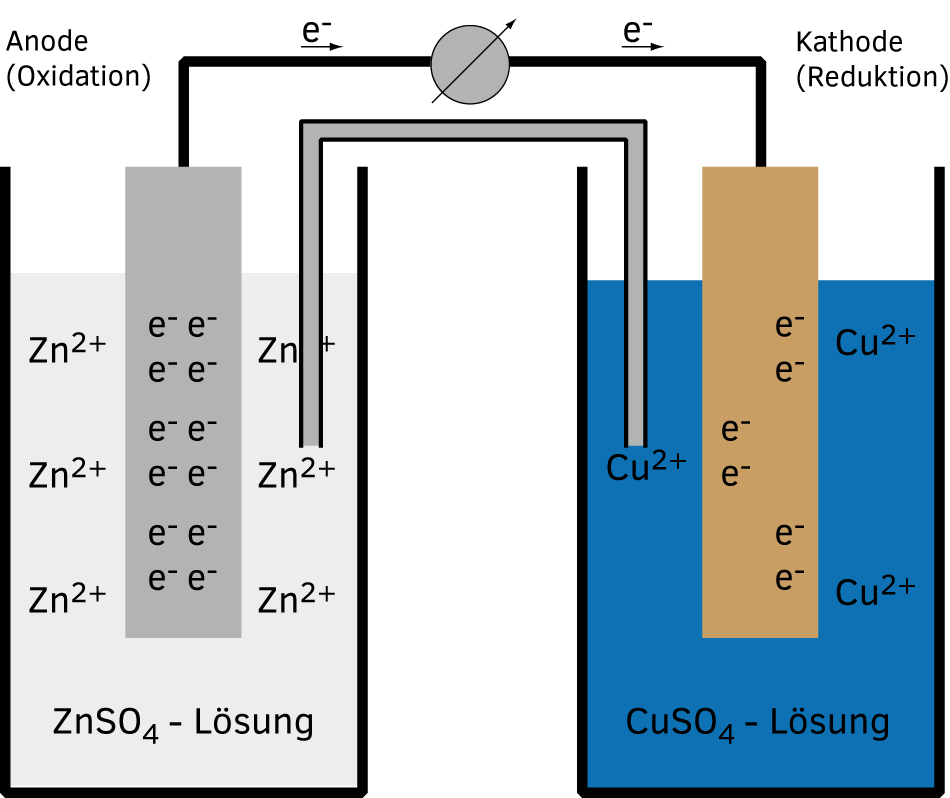
\includegraphics[width=0.7\linewidth]{skizzen/15/15_6/15_6B0}
\end{center}

offenes galvanisches Element

\begin{center}
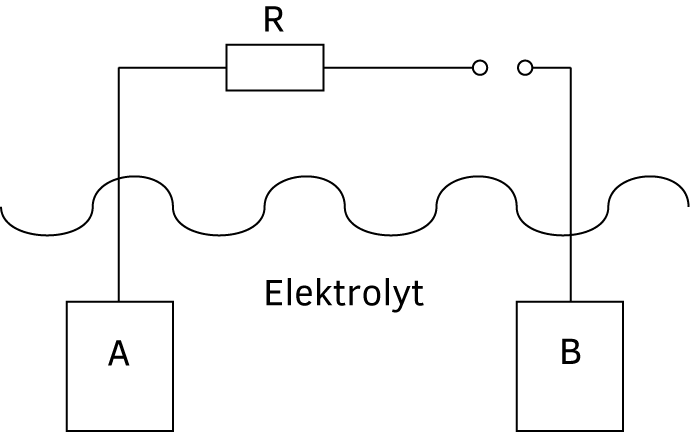
\includegraphics[width=0.4\linewidth]{skizzen/15/15_6/15_6B1}
\end{center}


\underline{innen}

\begin{center}
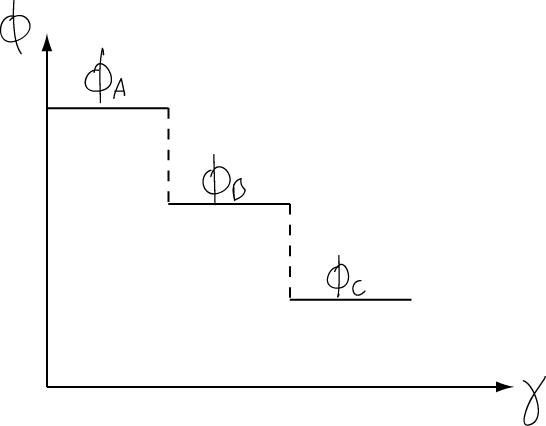
\includegraphics[width=0.5\linewidth]{skizzen/15/15_6/15_6B2}
\end{center}


\underline{außen}

\begin{center}
	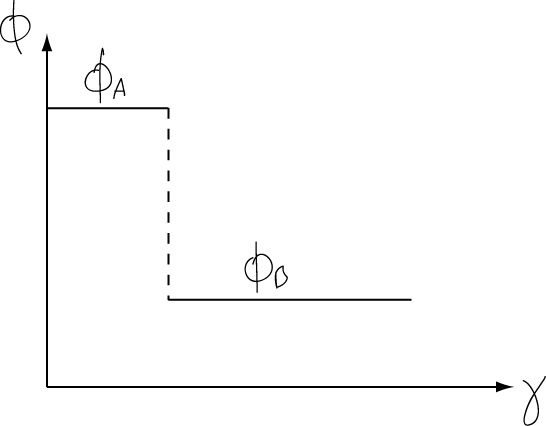
\includegraphics[width=0.5\linewidth]{skizzen/15/15_6/15_6B3}
\end{center}

$$ U_R = \phi_A-\phi_B = \underbrace{(\phi_A - \phi_{el}) + (\phi_{el}-\phi_B)}_{U_0\text{: Urspannung (Elektromotorische Kraft)}}  = U_0 $$

offenes galvanisches Element $ U_R = U_0 $

\hfill\break

Belastet

\begin{center}
	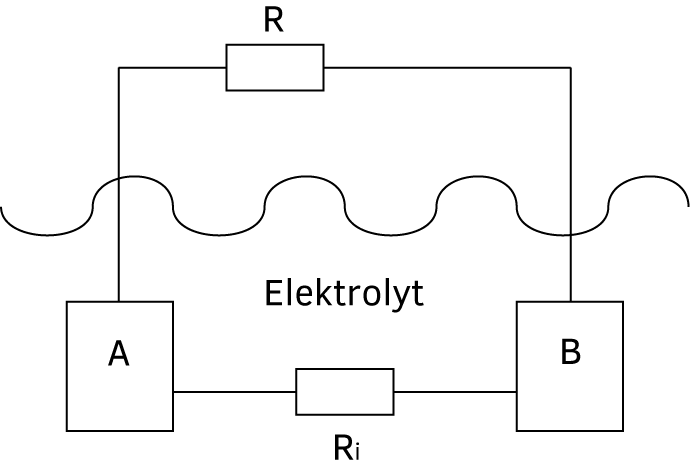
\includegraphics[width=0.4\linewidth]{skizzen/15/15_6/15_6B4}\\
	$ R_i $: Innenwiderstand
\end{center}



\underline{innen}

\begin{center}
	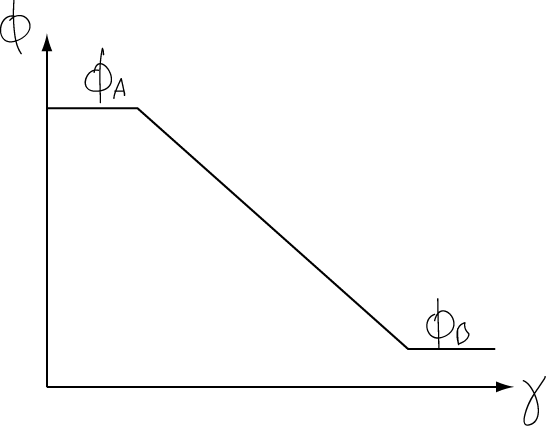
\includegraphics[width=0.5\linewidth]{skizzen/15/15_6/15_6B5}
\end{center}

\underline{außen}
\hypertarget{UR}{}
\begin{center}
	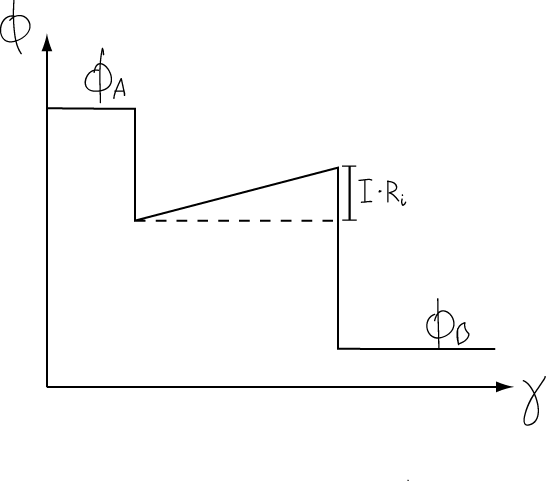
\includegraphics[width=0.5\linewidth]{skizzen/15/15_6/15_6B6}
\end{center}

$$ U_R = \phi_A-\phi_B = (\phi_A - \phi_{el}) - I \cdot R_i + (\phi_{el}-\phi_B) $$
$$ \boxed{U_R = U_0 - I \cdot R_i} $$

\begin{center}
	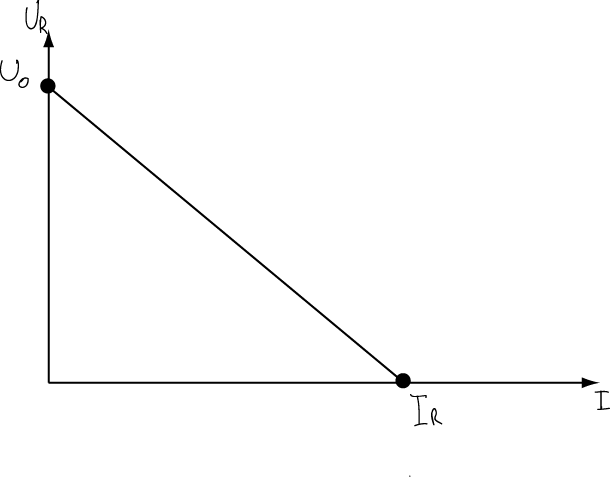
\includegraphics[width=0.5\linewidth]{skizzen/15/15_6/15_6B7}\\
	Kurzschlussstromstärke $ I_R = \frac{U_0}{R_I} $
\end{center}

Im Schaltbild:

\begin{center}
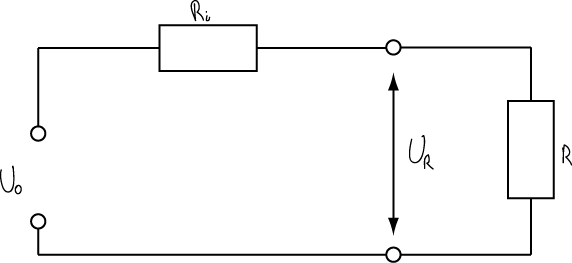
\includegraphics[width=0.6\linewidth]{skizzen/15/15_6/15_6B8}
\end{center}

\paragraph{Hilfe:}

\begin{itemize}
	\item Elektromotorische Kraft $ \equiv $ Urspannung \\
	Diese ist die Differenz $ E_{Kathode} - E_{Anode} = \Delta E  $\\
	Die Formale Definition ist $ \mathcal{E} = - {\displaystyle \int_{A}^{B} \vec{E}_{CS} \cdot d\vec{\ell} } $ \hspace{5mm}, wobei $ \vec{E}_{CS} $ das Elektro\underline{statische} Feld von/zwischen A und B ist. 
	\item Stromquellen werden häufig als Spannungsquelle bezeichnet bzw. diese ist gemeint
	\item An einer realen Spannungsquelle greift man die Klemmspannung ($ U_K $) ab. Diese ist \emph{nicht} gleich der Quellenspannung \hyperlink{UR}{(\textasteriskcentered)}
	\item Quellspannung wird hier als $ U_0 $ bezeichnet, häufiger aber $ U_Q $
	\item Klemmspannung wird hier als $ U_R $ bezeichnet, häufiger aber $ U_K $
\end{itemize}
